\documentclass[a4paper, twocolumn, twoside]{article}
\usepackage{amsmath}
\usepackage{amssymb}
\usepackage[backend=biber]{biblatex}
\usepackage{hyperref}
\usepackage{xcolor}
\usepackage{minted}
\usepackage{tikz}
\usepackage{listofitems}
\usepackage{amsmath}
\usepackage{tcolorbox}
\usepackage{etoolbox}
\usepackage[
	top=2cm, % Top margin
	bottom=2cm, % Bottom margin
	left=1.5cm, % Left margin
	right=1.5cm, % Right margin
	footskip=1cm, % Space from the bottom margin to the baseline of the footer
	headsep=0.75cm, % Space from the top margin to the baseline of the header
	columnsep=20pt, % Space between text columns (in twocolumn mode)
]{geometry}

\addbibresource{references.bib}

\BeforeBeginEnvironment{minted}{\begin{tcolorbox}}%
\AfterEndEnvironment{minted}{\end{tcolorbox}}%

\colorlet{myred}{red!80!black}
\colorlet{myblue}{blue!80!black}
\colorlet{mygreen}{green!60!black}
\colorlet{myorange}{orange!70!red!60!black}
\colorlet{mydarkred}{red!30!black}
\colorlet{mydarkblue}{blue!40!black}
\colorlet{mydarkgreen}{green!30!black}

\tikzset{
  >=latex, % for default LaTeX arrow head
  node/.style={thick,circle,draw=myblue,minimum size=22,inner sep=0.5,outer sep=0.6},
  node in/.style={node,green!20!black,draw=mygreen!30!black,fill=mygreen!25},
  node hidden/.style={node,blue!20!black,draw=myblue!30!black,fill=myblue!20},
  node convol/.style={node,orange!20!black,draw=myorange!30!black,fill=myorange!20},
  node out/.style={node,red!20!black,draw=myred!30!black,fill=myred!20},
  connect/.style={thick,mydarkblue}, %,line cap=round
  connect arrow/.style={-{Latex[length=4,width=3.5]},thick,mydarkblue,shorten <=0.5,shorten >=1},
  node 1/.style={node in}, % node styles, numbered for easy mapping with \nstyle
  node 2/.style={node hidden},
  node 3/.style={node out}
}
\def\nstyle{int(\lay<\Nnodlen?min(2,\lay):3)} % map layer number onto 1, 2, or 3

\tikzstyle{densenode}=[thick,draw=blue,fill=blue!20,circle,minimum size=22]
\tikzstyle{activationnode}=[thick,draw=red,fill=red!20,circle,minimum size=22]

\hypersetup{
    colorlinks,
    linkcolor={black},
    citecolor={blue!50!black},
    urlcolor={blue!80!black},
	frenchlinks=true,
}

\title{Deep learning: Neural Network from scratch\\
\textit{creating a neural network library to solve the mnist dataset}}
\author{Adrien PELFRESNE - Alexis VAPAILLE}
\date{\today}


\begin{document}
	\onecolumn
    \maketitle
	\tableofcontents

	\twocolumn
	\section{Abstract}
	\textit{We have created a deep neural network "library" from scratch, in rust, without the use of any machine learning or deep learning library.\\
	The goal of this project was to solve the mnist dataset of handwritten digits, and to provide performances comparaison between
	two multi-layer-perceptron, with and without convolution.\\
	Our library let you create your own sequential neural network, with a simple and declarative api and is widely open to extension.
	This project also include a drawing mode, when you can draw your own digit and see what the model guess.
	}

	\section{Motivation}
	Our motivation with this \textit{from scratch} approach was to deepen our understanding of neural networks.
	Because high level library like \href{https://keras.io/}{keras} and the incredible level of abstraction that come with it,
	let us sometimes forgot the inner machinery. Nevertheless,
	this underlying work that those library are doing is passionating, and we through it was a shame to be a simple user of those interface.\\
	The only (methematical) helper library that we have used is \href{https://crates.io/crates/ndarray}{ndarray}
	which provides an n-dimensional container for general elements
	and for numerics, as well of providing efficients matrix operations on the gpu.\\
	You can find our project on \href{https://github.com/dirdr/neural_network_from_scratch}{github}, we widely encourage reader to check the source code,
	as in this report, we won't go into code specific details and focus more on the abstract explanation.\\
	The workspace is split into multiple crates
	\begin{enumerate}
		\item The neural network library, under the crate \textit{nn\_lib}
		\item The mnist exemple, which is using the \textit{nn\_lib} to define the networks and benchmark the dataset, Under the crate mnist
		\item the gui code to run a interactive drawing mode is included in the workpsace in the app file.
	\end{enumerate}

	\section{Sequential neural network}
	The multi-layer perceptron is known  as a \textit{Sequential} neural network, meaning that the \textbf{output}
	$Y_N$ of the layer $L_N$ is the \textbf{input} $X_{N+1}$ of the next layer $L_{N+1}$.\\
	$$
	Y_{N} = X_{N+1}
	$$
	and conversely
	$$
	X_{N} = Y_{N-1}
	$$
	with subscript $N$ indentifying layers in sequential order.
	from the input layer, when we pass our data,
	through the output layer, data flows in the network, passing
	through different kind of layers.

	\subsection{General layer interface}
	We have defined a general \textit{Layer} interface, to be implemented by all the differents layer we gonna use.\\
	This interface has two main method : \textbf{feed\_forward} and \textbf{propagate\_backward},
	The \textit{feed forward} method take the input vector $X$ as parameter and return the output vector $Y$ of the layer.
	and the \textit{propagate backward} method take as parameters the layer output gradient $\frac{\partial C}{\partial Y}$ and return the layer input gradient $\frac{\partial C}{\partial X}$.
	We will cover the use of these function later, alongside the theorical explanation of these concepts.

	\subsection{Dense layer}
	A dense layer, also knowed as \textit{Linear layer}, is a layer where each input neuron is connected to every output neurone,
	each connexion is called a \textit{weight}, $w_{ij}$ is the weight
	connecting neurone $x_i$ (input) to neurone $y_j$ (output).

	\begin{figure}[H]
		\centering
		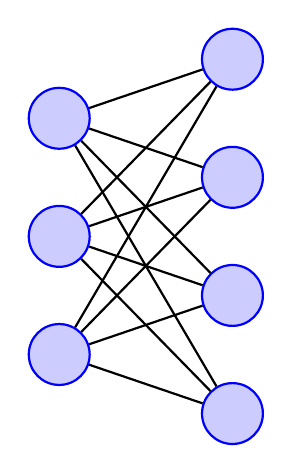
\begin{tikzpicture}[x=2.2cm,y=1.5cm]
		  \readlist\Nnod{3,4} % number of nodes per layer
		  % \Nnodlen = length of \Nnod (i.e. total number of layers)
		  % \Nnod[1] = element (number of nodes) at index 1
		  \foreachitem \N \in \Nnod{ % loop over layers
			% \N     = current element in this iteration (i.e. number of nodes for this layer)
			% \Ncnt  = index of current layer in this iteration
			\foreach \i [evaluate={\x=\Ncnt; \y=\N/2-\i+0.5; \prev=int(\Ncnt-1);}] in {1,...,\N}{ % loop over nodes
			  \node[densenode] (N\Ncnt-\i) at (\x,\y) {};
			  \ifnum\Ncnt>1 % connect to previous layer
				\foreach \j in {1,...,\Nnod[\prev]}{ % loop over nodes in previous layer
				  \draw[thick] (N\prev-\j) -- (N\Ncnt-\i); % connect arrows directly
				}
			  \fi % else: nothing to connect first layer
			}
		  }
		\end{tikzpicture}
	\caption{Dense Layer with 3 input nodes and 4 output nodes}
	\end{figure}
	
	We calculate a dense layer neuron output value $y_j$ as 
	$$
	y_j = \sum_{i=1}^{n} x_i w_{i,j} + b_j
	$$

	which is the bias corrected weighted sum of all the connected input nodes.
	$b_j$ is the bias term for the output neuron $j$.
	We can rewrite this operation to use matrix operation on whole vectors.

	$$
	Y = XW + B
	$$

	with $Y \in \mathbb{R}^j$, $X \in \mathbb{R}^i$, $W \in M_{i*j}(\mathbb{R})$ and $B \in \mathbb{R}^j$\\
	In this report, we will annotate vector like vector, but note that to
	be able to do the matmul in practice, a vector $X \in \mathbb{R}^i$ is actually broadcasted to a matrice $M_{1*i} (\mathbb{R})$

	\clearpage

	\subsection{Activation layer}
	There are two school of thought for defining activations.
	\begin{enumerate}
		\item activations are used to produce the output value \textbf{inside} a dense layer,
			in this case, the weighted sum of the dense layer is called $z$, and $y$ is calculated by applying
			an activation $\sigma$ to $z$ : $y : \sigma(z)$.
		\item activations are used \textbf{outside} dense layer  in this case,
			the output of a dense layer $y$ is equal to the weighted sum $z$.
			An activation Layer is used as a seperate layer,
			that applie the activation function to each neuron.
	\end{enumerate}

	We implemented our sequential neural network with the second paradigm,
	because it is actually easier in code to manage a dense and a activation
	layer separatly, mainly for backpropagation calculation ease.

	\begin{figure}[H]
	\centering
	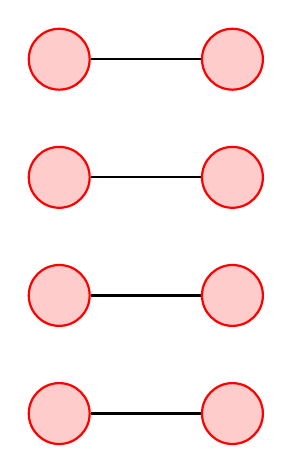
\begin{tikzpicture}[x=2.2cm,y=1.5cm]
	  \readlist\Nnod{4,4} % Define two layers, each with 4 nodes
	  % Loop over both layers
	  \foreachitem \N \in \Nnod{
		\foreach \i [evaluate={\x=\Ncnt; \y=\N/2-\i+0.5; \prev=int(\Ncnt-1);}] in {1,...,\N}{
		  \node[activationnode] (N\Ncnt-\i) at (\x,\y) {};
		  % If not the first layer, connect nodes from the previous layer
		  \ifnum\Ncnt>1
			\draw[thick] (N\prev-\i) -- (N\Ncnt-\i); % Connect nodes element-wise
		  \fi
		}
	  }
	\end{tikzpicture}
	\caption{Activation layer with 4 input neuron}
	\end{figure}

	The Activation layer take a vector $X \in \mathbb{R}^n$  as input and produce a vector $Y \in \mathbb{R}^n $ as output,
	with the activation function applied to each neuron.\\
	We must note that some activations function transform vector by
	mapping the vector individual components $x$ through the function, like ReLU

	$$
	ReLU(x) = max(0, x)
	$$

	While other activation functions, like \textit{softmax} work on whole vectors.
	Softmax take a vector $z \in \mathbb{R}^K$,
	convert it into a probability distribution of $K$ possible outcomes.

	$$
	\sigma : \mathbb{R}^{K} \rightarrow (0, 1)^K, K \geq 1
	$$

	is computed by taking a vector $z = (z_1, ..., z_k) \in \mathbb{R}^K$ and compute each component of a vector $\sigma(\mathbf{z}) \in (0, 1)^K$ 

	$$
	\sigma(\mathbf{z})_i = \frac{e^{z_i}}{\sum_{j = 1}^{K} e^{z_j}}
	$$

	Currents activations function implemented in our library are :
	\begin{itemize}
		\item{Sigmoid}
		\item{ReLU}
		\item{Tanh}
		\item{Softmax}
	\end{itemize}

	\section{Cost function}
	To mesure how well a neural network perform, we use a cost function, 
	which output a real number
	by comparing the neural network \textit{output}, 
	and the \textit{observed} value.\\
	A simple cost function is the meaned squared error :

	$$
	\text{MSE} = \frac{1}{n} \sum_{i=1}^{n} (\hat{y}_i - y_i)^2
	$$

	The MSE function is great for regression neural network when we want to predict a continuous value from a input.
	To do classification, like in the mnist data of handwritten digit,
	we use another cost function,
	the cross entropy cost function :

	$$
		\text{Cross Entropy} = -\sum_{c=1}^{C} y_{c} \log(\hat{y}_{c})
	$$

	with $C$ the number of class (eg: 10 for the mnist dataset), $y_{c}$ 
	the observed probability, and $\hat{y}_{c}$ the neural network output.\\
	This expression simpifie as

	$$
		\text{Cross Entropy} = -\log(\hat{y}_{c})
	$$

	if $y_{c}$ is one hot encoded (ie: 1 for the observed class and 0 for others).

	\section{The learning process}
	\subsection{Gradient}
	The gradient of a function $\nabla f$ is the vector field that represents the direction
	and rate of the quickest increase of the function from a point $p$.\\
	We can visualize the gradient and the curve of a function $f(x, y) = -(\cos^2 x  +\cos^2 y)^2$\\

	\begin{figure}[H]
		\begin{center}
			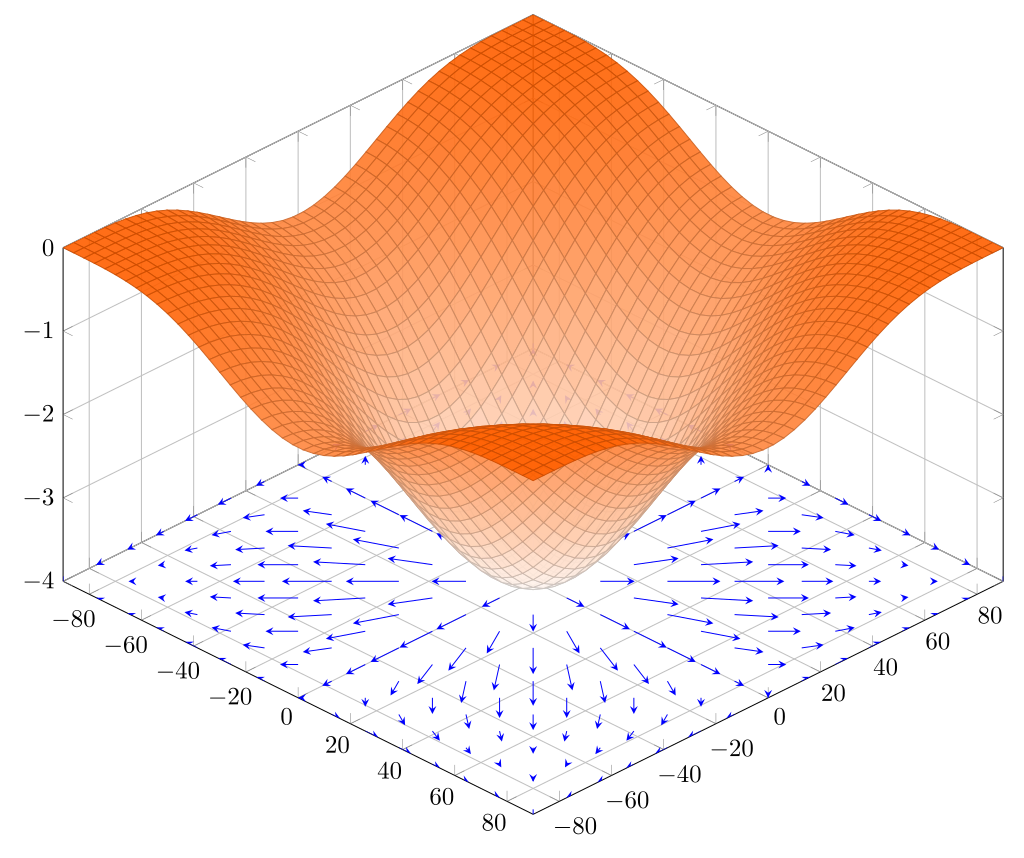
\includegraphics[width=\columnwidth]{images/gradient_2d.png}
		\end{center}
		\caption{Function representation and gradient field of the function $-(\cos^2 x  +\cos^2 y)^2$}\label{fig:gradien2d}
	\end{figure}

	The field vector below the function curve represent the gradient,
	for each point $p = (x, y)$ the arrow at $p$ point toward the direction
	with the fastest increase of $f$.

	\subsection{Minimization}
	To make our neural network lean, we adjust his parameters (ie: weights and biases for a dense layer)
	to \textbf{minimize the cost function $C$ of the network}.
	We can use the cost function gradient, which tell us the direction and magnitude
	of the fastest \textbf{increase} of cost, and proceed to go in the opposite direction,
	which will make us go toward the fastest \textbf{decrease} of the cost function.\\
	The algorithm used to minimize the cost function is the \textit{gradient descent},
	which will repeatedly descent the curve by going toward the opposite of the gradient of the cost function.

	Here is the process for a signle gradient descent step :
	\begin{enumerate}
		\item feed all input data points into the network,
			calculating the cost for every output.
		\item calculate the averaged cost.
		\item compute the gradient of the averaged cost function \textbf{with respect to the network parameters}.
		\item update the parameters in the opposite direction of the gradient
	\end{enumerate}

	\subsection{backpropagation}
	To do a gradient descent step, we need the gradient of
	the cost function with respect to the neural network parameters,
	the algorithm used to calculate this gradient 
	is called \textbf{backpropagation}.\\
	Backpropagation precisely calculate
	(and not only estimate like the finite difference method) the gradient of the cost function $C$ with respect to the neural network parameters,
	that we will call parameters gradient $\frac{\partial C}{\partial P}$.\\
	For each layer $L$, we calculate the gradient with respect to the parameters of $L$,
	starting from the last layer $L_n$ and going all the way back to the first layer $L_0$.\\
	The key methematical tool used in backpropagation is the chain rule,
	which allow the gradient of the cost function
	to be split into gradient of simpler functions at each neuron within the network.\\
	For each layer $L_n$, to calculate the parameters gradient $\frac{\partial C}{\partial P_n}$,
	we need to know the output gradient $\frac{\partial C}{\partial Y_n}$, this gradient is given to us by the next layer in the sequential order,
	because in the sequential architecture $\frac{\partial C}{\partial X_{n+1}} = \frac{\partial C}{\partial Y_n}$.
	We want to also calculate $\frac{\partial C}{\partial X_i}$, the input $X$ gradient,
	to transmit it to the previous layer, which need it to calculate her own parameters gradient $\frac{\partial C}{\partial W_{i-1}}$.\\
	You can probably feel why this process is called backpropagation, we are sharing gradient,
	from layer to layer, starting at the last layer and going back up to the start of the net.
	Each layer implementation will have a specific implementation of the \textbf{propagate backward method},
	in the next sections, we will cover the calculation for the layer we used in our library.

	\subsection{Dense layer backpropagation}

	The dense layer have two trainable parameters, the weigths, $W$ and the biases $B$.
	Starting with the gradient of the cost function with respect to the weights, we are given
	the output gradient :

	\begin{align}
		\frac{\partial C}{\partial Y} &= \begin{bmatrix}
		\frac{\partial C}{\partial y_1} \\
		\frac{\partial C}{\partial y_2} \\
        \vdots \\
	   \frac{\partial C}{\partial y_j} \\
	\end{bmatrix}
	\end{align}

	The cost function $C$ depend on $Y$ which depend on $W$ thus $C$ depend on $W$ (chain rule)

	$$
    \frac{\partial C}{\partial W} = \frac{\partial C}{\partial Y} \frac{\partial Y}{\partial W}
	$$

	We calculate each weight gradient component $\frac{\partial C }{\partial W_{ij}}$

	$$
    \frac{\partial C}{\partial W_{ij}} = \sum_{l=1}^{N} \frac{\partial L}{\partial Y_{lj}} \frac{\partial Y_{lj}}{\partial W_{ij}}
	$$

	because $W_{ij}$ is used in every example for calculating the $j^{th}$ column of the output matrix. Let's look at the formula for $Y_{lj}$ to get the derivative

	$$
		Y_{lj} = X_{l1}W_{1j} + \cdots + X_{li}W_{ij} + \cdots + X_{lp}W_{pj} + b_{j}
	$$
	$$
		\frac{\partial Y_{lj}}{\partial W_{ij}} = X_{li}
	$$
	$$
		\implies \frac{\partial C}{\partial W_{ij}} = \sum_{l=1}^{N} \frac{\partial C}{\partial Y_{lj}} X_{li} = \sum_{l=1}^{N} X^{T}_{il}\frac{\partial C}{\partial Y_{lj}}
	$$

	So finally 

	$$
		\frac{\partial C}{\partial W} = X^{T} \frac{\partial C}{dY}
	$$

	for the biases $B$.

	\begin{align}
		\frac{\partial C}{\partial b} &= \frac{\partial C}{\partial Y} \frac{\partial Y}{\partial b}\\
		\frac{\partial C}{\partial b_{i}} &= \sum_{l=1}^{N} \frac{\partial C}{\partial Y_{li}} \frac{\partial Y_{li}}{db}
	\end{align}

	since the bias term $b_{i}$ is used in the evaluation of the entire column of $Y$.

	$$
		\frac{\partial Y_{li}}{\partial b_{i}} = 1
	$$
	$$
		\frac{\partial C}{db_{i}} = \sum_{l=1}^{N} \frac{\partial C}{\partial Y_{li}}
	$$
	$$
		\frac{\partial C}{\partial b} = \frac{\partial C}{\partial Y}
	$$

	and lastly, we calculate the gradient with respect to $X$

	\begin{align}
		\frac{\partial C}{\partial X} &= \frac{\partial C}{\partial Y} \frac{\partial Y}{\partial X}\\
		\frac{\partial C}{\partial X_{ij}} &= \sum_{l=1}^{k} \frac{\partial C}{\partial Y_{il}} \frac{\partial Y_{il}}{\partial X_{ij}}
	\end{align}

	since the data point $i$ will only influence the data point $i$ in $Y$. Other data points will not be affected. Further, $X_{ij}$ is used in calculation of every dimension of $Y_{i,:}$. To calculate the gradient,

	$$
		Y_{il} = \sum_{t=1}^{p} X_{it}W_{tl}
	$$
	$$
		\frac{\partial Y_{il}}{\partial X_{ij}} = W_{jl}
	$$
	$$
		\frac{\partial C}{\partial X_{ij}} = \sum_{l=1}^{k} \frac{\partial C}{\partial Y_{il}}W_{jl}
		= \sum_{l=1}^{k} \frac{\partial C}{\partial Y_{il}} W_{lj}^{T}
	$$
	$$
		\implies \frac{\partial C}{\partial X} = \frac{\partial C}{\partial Y} W^{T}
	$$

	\subsection{Activation layer backpropagation}

	An activation layer doesn't have any trainable parameters, so we just gonna focus on the input gradient calculation.

	we are given
	the output gradient $\frac{\partial C}{\partial Y}$:
	we know that 

	\begin{align*}
		Y &= \begin{bmatrix}
		f(X_1) \\
		f(X_2) \\
        \vdots \\
		f(X_i)
	\end{bmatrix}
	\end{align*}

	$$
    \frac{\partial C}{\partial X} = \frac{\partial C}{\partial Y} \frac{\partial Y}{\partial X}
	$$

	$$
    \frac{\partial C}{\partial X_{ij}} = \sum_{l=1}^{N} \frac{\partial C}{\partial Y_{lj}} \frac{\partial Y_{lj}}{\partial X_{ij}}
	$$

	using the same procedure as for the previous calculations

	$$
	\implies \frac{\partial C}{\partial X} = \frac{\partial C}{\partial Y} \odot Y\prime
	$$

	with 

	\begin{align*}
		Y\prime &= \begin{bmatrix}
		f\prime(X_1) \\
		f\prime(X_2) \\
        \vdots \\
		f\prime(X_i)
	\end{bmatrix}
	\end{align*}

	\section{Optimizers}
	
	At this point, to updates a neural network parameter $\theta$, we the gradient descent formula,
	with a fix learning rate $\eta$

	$$
	\theta := \theta - \eta \frac{\partial C}{\partial \theta}
	$$

	This is know, in the keras api for exemple as the \textit{Stochastic gradient descent optimizer},
	but it exist other optimizers such as \textit{Adam}.

	\subsection{Adam}
	Adam accelerate the convergence towards the optimal set of weights by taking into account passed gradient,
	and adam will adapt the learning rate for each individual weight.

	ADAM initializes two vectors, 
	$m$ and $v$, which store the exponential moving averages of past gradients and past squared gradients,
	respectively. These vectors are used to scale the gradient updates adaptatively.

	\begin{enumerate}
	  \item \textbf{Initialization:} Initialize two vectors, $m$ and $v$, to store the moving averages of the gradients and their squares, respectively.
	  \item \textbf{Computing Moving Averages of the Gradients:}
		\begin{align*}
		  m_t &= \beta_1 \cdot m_{t-1} + (1 - \beta_1) \cdot g_t, \\
		  v_t &= \beta_2 \cdot v_{t-1} + (1 - \beta_2) \cdot g_t^2,
		\end{align*}
		where $g_t$ is the gradient at time step $t$, and $\beta_1$ and $\beta_2$ are factors that control the decay rates.
	  \item \textbf{Bias Correction:} Correct initial bias in $m$ and $v$:
		\begin{align*}
		  \hat{m}_t &= \frac{m_t}{1 - \beta_1^t}, \\
		  \hat{v}_t &= \frac{v_t}{1 - \beta_2^t}.
		\end{align*}
	  \item \textbf{Update Weights:} Adjust weights based on the corrected moments:
		\begin{equation*}
		  \theta_{t+1} = \theta_t - \frac{\eta}{\sqrt{\hat{v}_t} + \epsilon} \cdot \hat{m}_t,
		\end{equation*}
		where $\theta$ are the parameters, $\eta$ is the learning rate, and $\epsilon$ is a small constant for numerical stability.
	\end{enumerate}

	\section{Batching}
	We went through several feed forward implementations. The first one was to pass data point one by one in the network
	$x \in \mathbb{R}^{i}$\dots. This was very slow, for exemple, for the mnist dataset, which has 60k training exemples,
	we where going through the whole neural network : feed forward, cost evaluation, back propagation, 60k times.
	But we then leraned that we can instead pass \textit{batch} of data in the neural network, in one time, and this batch can
	be of any length.
	the input then becomes $x \in M_{nxi} (\mathbb{R})$ with each line of the input matrice representing a single data point.

	The calculation became much faster, because we can now feed $n$ element at a time in the neural network.

	\section{Initializer}
	Initializers determine the starting weights of a neural network, it is important to choose the right initializer, depending
	on our netwrok architecture, to avoid problem like vanishing and exploding gradient, and to also optimizer convergence.

	At the moment we are writing this report, we have imoplemented two initializer inside our library,

	\begin{enumerate}
		\item{he}
	The He initializer, designed for ReLu activation functions,
	initializes weights from a normal distribution centered at zero with a standard deviation of 
	$\sqrt{\frac{2}{n}}$ (where $n$ is the number of input nodes).
	This setup helps prevent the vanishing gradient problem in deep networks with ReLu activations,
	ensuring that gradients remain large enough to sustain effective learning through many layers.
		\item{Glorot uniform}
	Conversely, the GlorotUniform initializer, 
	also known as Xavier Uniform, is ideal for networks using sigmoid or tanh activations.
	It selects weights from a uniform distribution within $[-c, c]$,
	where $c = \sqrt{\frac{6}{n_{\text{in}} + n_{\text{out}}}}$.
	This approach maintains a balance in the variance of neurons' outputs across the network,
	aiding in stable gradient flow in deep networks with saturating activations.
	\end{enumerate}

	\section{Convolutional neural network}
	ALEXIS a toi de travailler

	\section{Metrics}
	With the mnist datset, which is a classification problem, we can implements multiple metrics
	to evaluate the network performances, we will explain the one we implemented in our library.

	\begin{enumerate}
		\item Accuracy measures the proportion of correct prediction to the total observations in the dataset.
		for exemple if we have correctly classified 950 image out of 1000, the accuracy will be 95percent.
		$$
		\text{Accuracy} = \frac{\text{Number of Correct Predictions}}{\text{Total Number of Predictions}}
		$$

		Precision and Recall are two metrics acting on a specified class.
		\textbf{Retrieved elements} are all the network prediction for a specific class.
		\textbf{Relevant elements} are all the correct instances of 
		the class \cite{wiki_precision_recall}.

		\item Precision answer the question : \textit{How many retrieved items are relevant}
		$$
		\text{Precision} = \frac{\text{Relevant retreived instance}}{\text{All retrieved instance}}
		$$
		\item Recall answers the question: \textit{How many relevant item are retrieved}
		$$
		\text{Recall} = \frac{\text{Relevant instances}}{\text{All relevants instance}}
		$$
	\end{enumerate}

	\section{Training, Validation, and Test Sets}
	To monitor the performances of a neural network effectively,
	it is important to break down the dataset into three distinct subsets:
	training, validation, and test sets.

	\begin{itemize}
\item{\textbf{Training set}} : The training set is used during the leraning phase,
	with training data directly influencing the parameters updates
\item{\textbf{Validation set}} : The validation set is used to provide an unbiased evaluation of a model fit
	on the training dataset while tuning the model's hyperparameters.
	This set is used during training, to prevent overfitting when the model performs well on the training data
	but poorly on unseen data.
\item{\textbf{Test set}} :	The test set is used only after the model's training and validation phases are complete.
	It provides the final, unbiased performance metric of the neural network.
	\end{itemize}

	\section{Results}
	We include a small code snippet, showing our custom library api to declare a sequential neural network.

	\begin{minted}[breaklines, tabsize=2]{rust}
let net = NeuralNetworkBuilder::new()
	.push(DenseLayer::new(
		28 * 28,
		32,
		InitializerType::He,
	))
	.push(
		ActivationLayer::from(Activation::ReLU)
	)
	.push(
		DenseLayer::new(32, 10, InitializerType::He)
	)
	.push(
		ActivationLayer::from(
			Activation::Softmax
		)
	);
	.watch(MetricsType::Accuracy)
	.watch(MetricsType::Precision)
	.watch(MetricsType::Recall)
Ok(net.compile(GradientDescent::new(0.01), CostFunction::CrossEntropy)?)
	\end{minted}

	the layer are added in sequential order with the push method, we watched Accuracy, Precision and Recall.
	the \textit{watch} method will add a \textit{MetricsType} to the list of metrics that the program need to calculate.
	those metrics can be given over epochs for the training and validation dataset. and for the test dataset.

	To create a great network, we will try to reach the \textit{VC trade-off principle} \cite{LeCun2019} \cite{vapnik1974theory},
	this principle state that:

	\begin{enumerate}
		\item A more complex model might fit the training data very well (low training error)
			but risks overfitting, meaning it could perform poorly on new data
			because it is too tailored to the training set (high variance).
		\item A less complex model might not fit the training data as closely 
			(higher training error) but can generalize better on new data because 
			it does not capture the noise and specific details of the training set (low variance).
	\end{enumerate}

	Our challenge will thus be, to find the right level of complexity that minimizes both the error on the training data.

	\subsection{Multi-layer perceptron}
	before trying to get a great fitting model, we will anlyse the result of an overfitting model, to see 
	how this behavior translate into metrics. To make a model overfit, we have multiple options

	\begin{itemize}
		\item increase the model complexity (number of hidden layers, number of neuron per layer)
		\item reduce the batch size to make the learning process very granular 
			and increase the chance of the network leraning to much specific patterns
	\end{itemize}

	In our case we have choosen to lower the batch size, here is our network hyperparameters

	\begin{table}[H]
	\centering
	\begin{tabular}{|l|c|c|}
	\hline
	hyperparameters & epochs & batch size  \\
	\hline
	Value & 30 & 5   \\
	\hline
	\end{tabular}
	\caption{hyperparameters overfitting model}
	\end{table}

	\begin{figure}[H]
		\begin{center}
			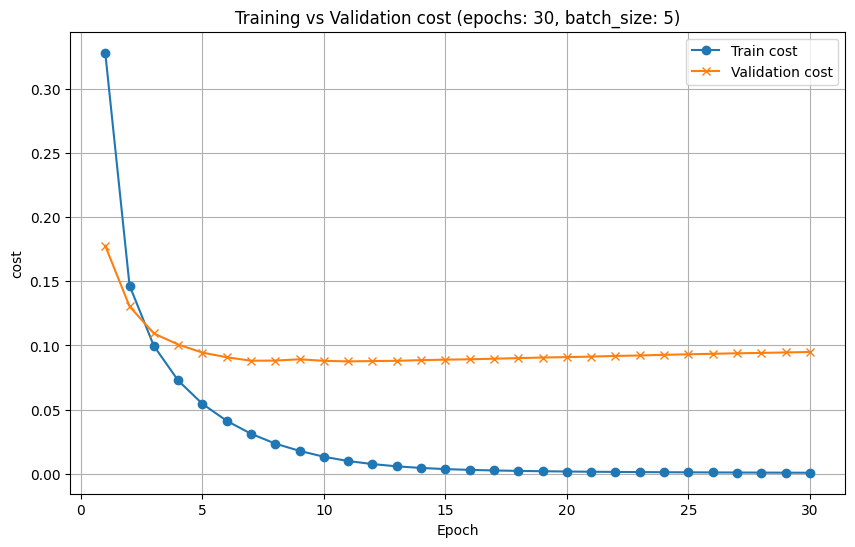
\includegraphics[width=\columnwidth]{images/cost_overfit.png}
		\end{center}
		\caption{Training vs Validation cost overfitting model}\label{fig:cost_overfit}
	\end{figure}

	In the cost comparaison between our training data and our validation data, the overfitting
	clearly stand out, our train cost (or loss) get very low, while the validation cost remain stable
	this mean that our neural network has learn to much specific pattern in the training data,
	making the error going very low on this set, but on the validation set, the network
	doesn't achieve a great generalization.

	\begin{figure}[H]
		\begin{center}
			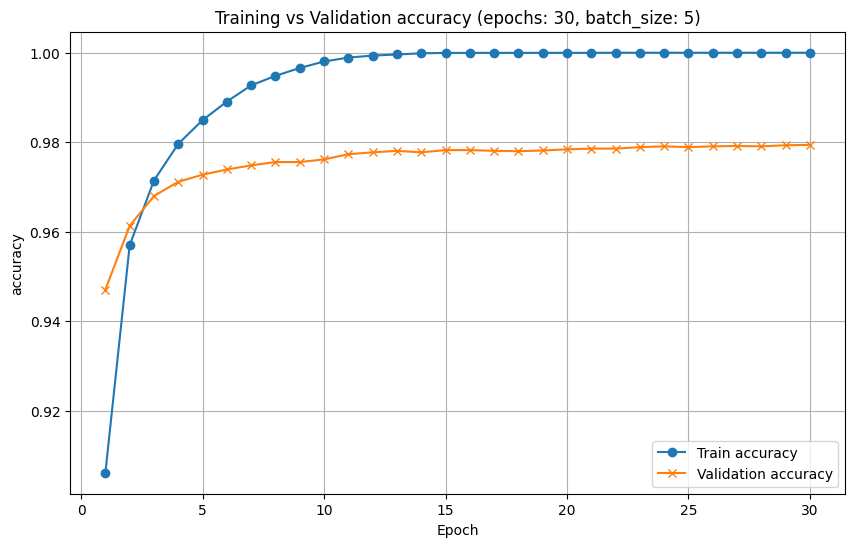
\includegraphics[width=\columnwidth]{images/accuracy_overfit.png}
		\end{center}
		\caption{Training vs Validation cost overfitting model}\label{fig:accuracy_overfit}
	\end{figure}

	The same observation applies to the evolution of accuracy over epochs.
	the accuracy reach a stunning 100percent on our training data, meaning that with
	the point used to train the network, it dont make any mistakes,
	but the validation accuracy struggle to get up.\\

	We have achieved our best accuracy with the following hyperparameters and network definition.

	\begin{table}[H]
	\centering
	\begin{tabular}{|l|c|c|}
	\hline
	hyperparameters & epochs & batch size  \\
	\hline
	Value & 15 & 100   \\
	\hline
	\end{tabular}
	\caption{hyperparameters greatfitting model}
	\end{table}


	\begin{minted}[breaklines, tabsize=2]{rust}
let net = SequentialBuilder::new()
	.push(
		DenseLayer::new(784, 256,
		InitializerType::He))
	.push(
		ActivationLayer::from(
			Activation::ReLU)
		)
	.push(
		DenseLayer::new(256, 256,
		InitializerType::He))
	.push(
		ActivationLayer::from(
			Activation::ReLU)
		)
	.push(
		DenseLayer::new(256, 10,
		InitializerType::GlorotUniform))
	.push(
		ActivationLayer::from
		(
			Activation::Softmax)
		)
	.watch(MetricsType::Accuracy);
Ok(net.compile(GradientDescent::new(0.04), CostFunction::CrossEntropy)?)
	\end{minted}


	\begin{figure}[H]
		\begin{center}
			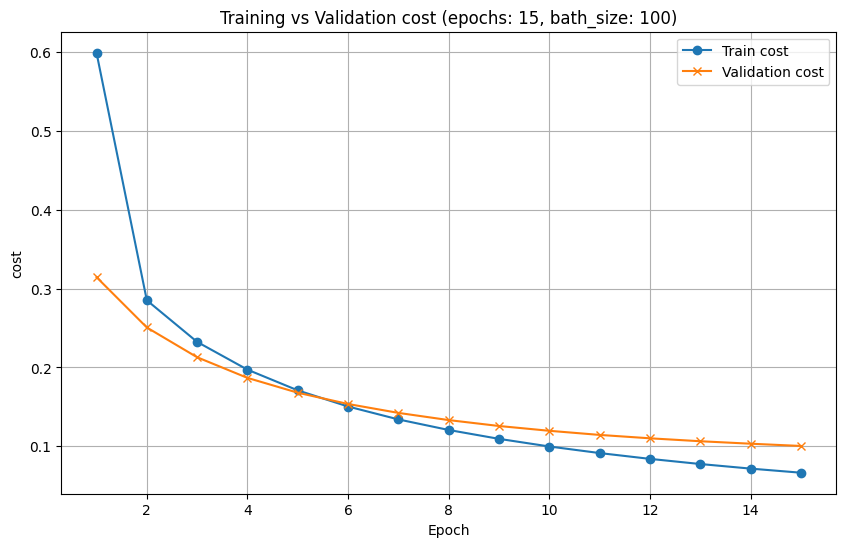
\includegraphics[width=\columnwidth]{images/cost_greatfit.png}
		\end{center}
		\caption{Training vs Validation cost greatfitting model}\label{fig:cost_greatfit}
	\end{figure}

	Here, our model seems to have generalized patterns, because the training cost and 
	the validation cost follow the same path, slowly increasing, with the gap between curves never blowing off the roof.

	we reach a validation cost of 0.097, the cost for the testing data set is 0.091.

	\begin{figure}[H]
		\begin{center}
			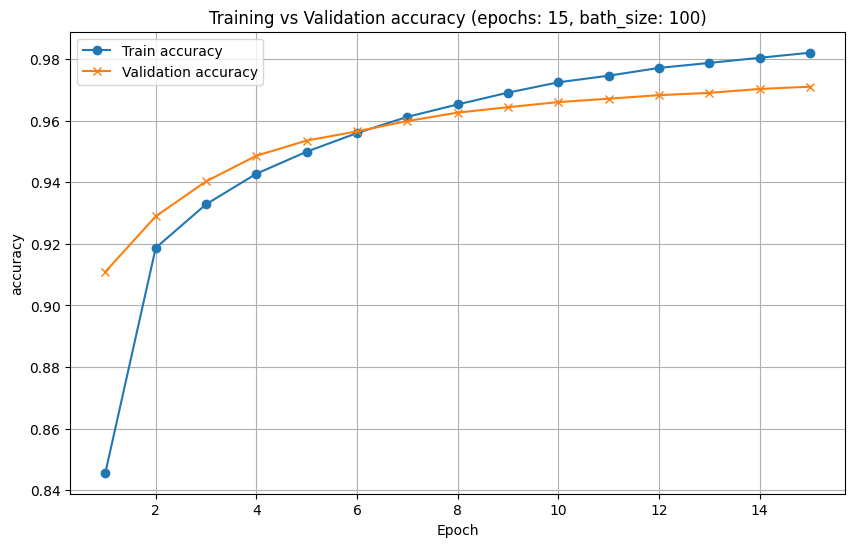
\includegraphics[width=\columnwidth]{images/accuracy_greatfit.png}
		\end{center}
		\caption{Training vs Validation cost greatfitting model}\label{fig:accuracy_greatfit}
	\end{figure}

	we reach a validation accuracy of 97.10percent for the final eppochs, the accuracy for the testing data set is 97.31percent.
	which is not a \textit{state of the art} accuracy but is a good result.

	\subsection{Convolutional multi-layer perceptron}

	\section{Conclusion}
	This project of creating our own \textit{from scratch} library has brought us a lot of knowledge,
	It as made us greatly understand the whole neural network process.
	We have planned to add more functionality to our library and to optimize the code base even after the end of this project.
	we want to add more optimizers, the dropout layer, and a learning rate scheduler.
	and over the longer term, we'd like to add other neural network paradigm, such as Recurrent neural network.

	\nocite{*}
	\printbibliography

\end{document}
